\documentclass[11pt]{article}
\usepackage{geometry} % Pour passer au format A4
\geometry{hmargin=1cm, vmargin=1cm} % 

% Page et encodage
\usepackage[T1]{fontenc} % Use 8-bit encoding that has 256 glyphs
\usepackage[english,french]{babel} % Français et anglais
\usepackage[utf8]{inputenc} 

\usepackage{lmodern}
\setlength\parindent{0pt}

% Graphiques
\usepackage{graphicx,float,grffile}
\usepackage{pstricks,pst-plot,pst-text,pst-tree,pstricks-add,pst-3d}

% Maths et divers
\usepackage{amsmath,amsfonts,amssymb,amsthm,verbatim,tabularx}
\usepackage{multicol,enumitem,url,eurosym,gensymb,multido}

% Sections
\usepackage{sectsty} % Allows customizing section commands
\allsectionsfont{\centering \normalfont\scshape}

% Tête et pied de page

\usepackage{fancyhdr} 
\pagestyle{fancyplain} 

\fancyhead{} % No page header
\fancyfoot{}

\renewcommand{\headrulewidth}{0pt} % Remove header underlines
\renewcommand{\footrulewidth}{0pt} % Remove footer underlines

\newcommand{\horrule}[1]{\rule{\linewidth}{#1}} % Create horizontal rule command with 1 argument of height

%----------------------------------------------------------------------------------------
%   Début du document
%----------------------------------------------------------------------------------------

\begin{document}

%----------------------------------------------------------------------------------------
% RE-DEFINITION
%----------------------------------------------------------------------------------------
% MATHS
%-----------

\newtheorem{Definition}{Définition}
\newtheorem{Theorem}{Théorème}
\newtheorem{Proposition}{Propriété}

% MATHS
%-----------
\renewcommand{\labelitemi}{$\bullet$}
\renewcommand{\labelitemii}{$\circ$}
%----------------------------------------------------------------------------------------
%   Titre
%----------------------------------------------------------------------------------------

\setlength{\columnseprule}{1pt}

\horrule{2px}
\section*{Chapitre 3 - Espace}
\horrule{2px}
\vspace{-1cm}

\subsubsection*{Exercice 1 - Vase}

Antoine crée des objets de décoration avec des vases, des billes et de l’eau colorée. Pour sa nouvelle création, il décide d’utiliser le vase et les billes ayant les caractéristiques suivantes :

\begin{figure}[H]
      \centering
      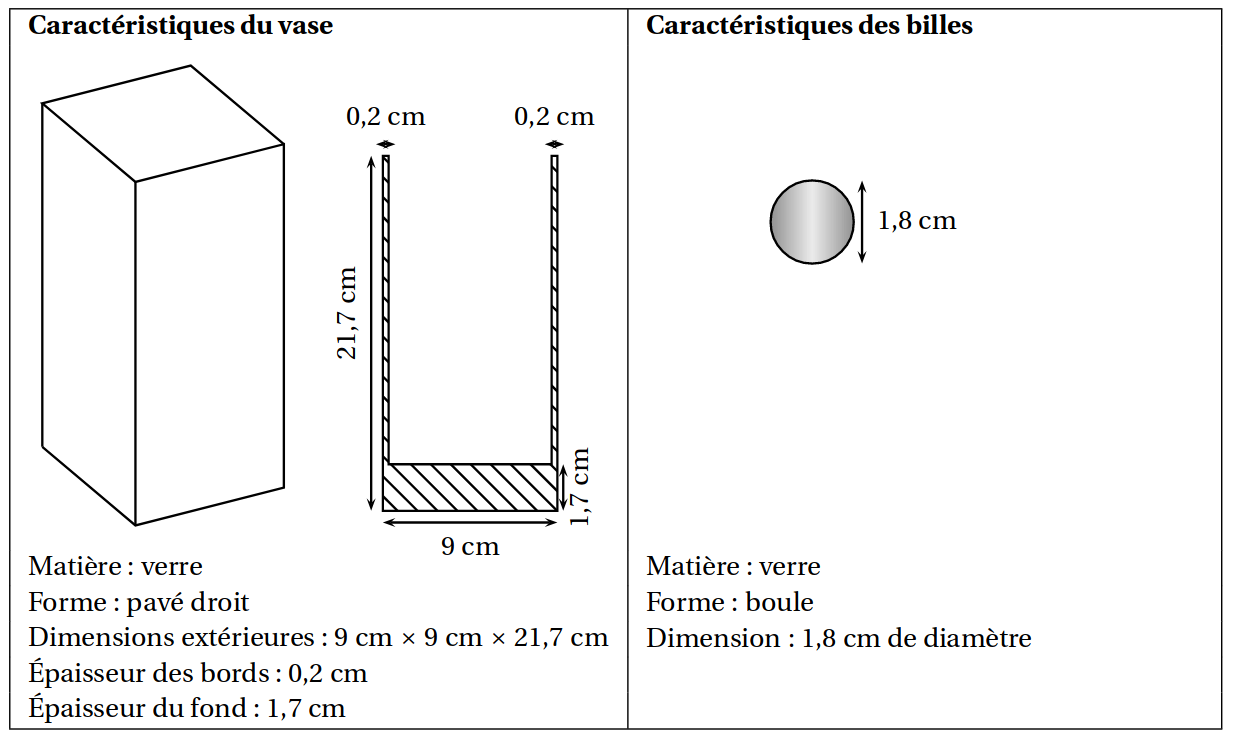
\includegraphics[width=0.7\linewidth]{3x3-volumes-1/sources/bille.png}
\end{figure}

\textbf{Il met 150 billes dans le vase. Peut-il ajouter un litre d’eaucolorée sans risquer le débordement ?}

Rappels : 

\begin{itemize}
\item Volume de la sphère = $\dfrac{4}{3} \times \pi  \times rayon^3$
\end{itemize}

\subsubsection*{Exercice 2 - Sel}

La fleur de sel est la mince couche de cristaux blancs qui se forme et affleure la surface des maraissalants. Chaque soir, Jean cueille la fleur de sel à la surfacedes carreaux. Pour transporter sa récolte,il utilise une brouette comme sur le schéma ci-dessous.

\begin{figure}[H]
      \centering
      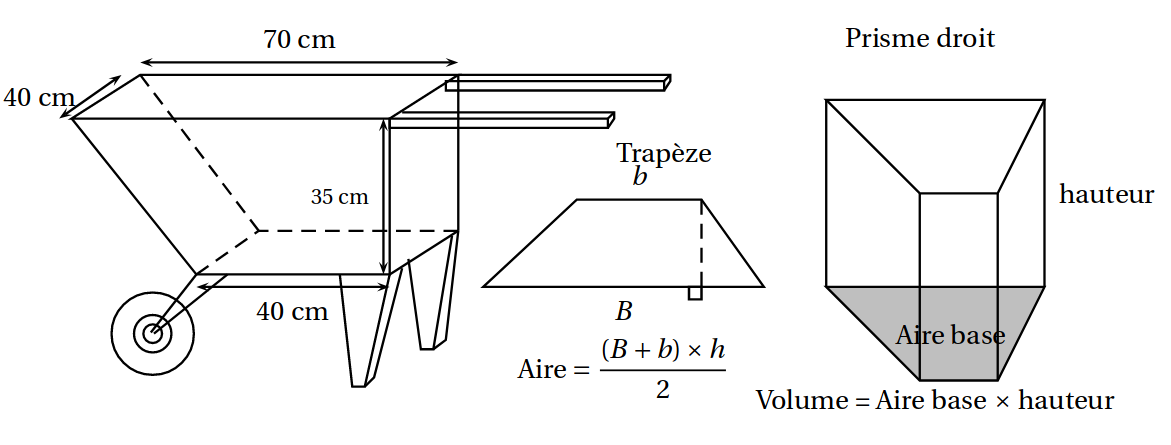
\includegraphics[width=0.8\linewidth]{3x3-volumes-1/sources/brouette.png}
\end{figure}

\begin{enumerate}
\item Montrer que cette brouette a un volume de 77 litres.
\item Sachant que 1 litre de fleur de sel pèse 900 grammes, calculer la masse en kg du contenu d’unebrouette remplie de fleur de sel
\end{enumerate}

\newpage

\subsubsection*{Exercice 3 - boulet}

Pour ranger les boulets de canon, les soldats du $XVI^e$ siècle utilisaient souvent un type d’empilement pyramidal à base carrée, comme le montrent les dessins suivants :

\begin{figure}[H]
      \centering
      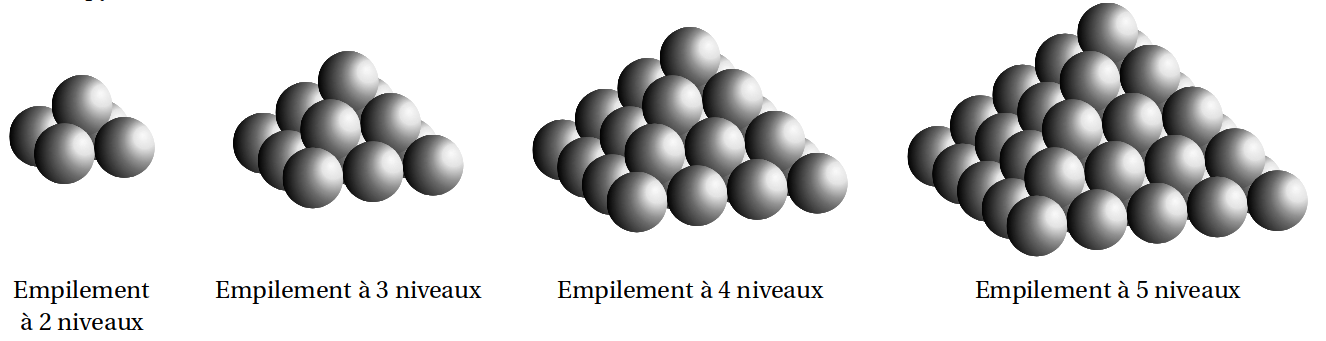
\includegraphics[width=0.8\linewidth]{3x3-volumes-1/sources/boules.png}
\end{figure}

\begin{enumerate}
\item Combien de boulets contient l’empilement à 2 niveaux ?
\item Expliquer pourquoi l’empilement à 3 niveaux contient 14 boulets
\item On range 55 boulets de canon selon cette méthode. Combien de niveaux comporte alors l’em-pilement obtenu?
\item Ces boulets sont en fonte; la masse volumique de cette fonte est de $7300kg/m^3$. On modélise un boulet de canon par une boule de rayon 6cm. Montrer que l’empilement à 3 niveaux de ces boulets pèse 92kg, au kg près.
\end{enumerate}

Rappels : 

\begin{itemize}
 \item volume d’une boule = $\dfrac{4}{3} \times \pi \times Rayon^3$.
 \item une masse volumique de $7300kg/m^3$ signifie que $1m^3$ pèse 73 kg
\end{itemize}


\subsubsection*{Exercice 4 - Globe}

\begin{multicols}{2}

  \begin{enumerate}
  \item On considère que ce globe est composé d’un cylindre en cristal de diamètre 6cm, surmonté d’une boule de cristal. Voir schéma ci-contre. Montrer qu’une valeur approchée du volume de la boule de ce trophée est de $6 371 cm^3$
  \item Marie affirme que le volume de la boule de cristal repré-sente environ 90\% du volume total du trophée. A-t-elle raison ?
  \end{enumerate}

  Rappels : 

  \begin{itemize}
  \item Volume d’une boule = $\dfrac{4}{3} \times \pi \times rayon^3$
  \item volume d’un cylindre = $\pi \times rayon^2 \times hauteur$
  \end{itemize}

  \begin{figure}[H]
        \centering
        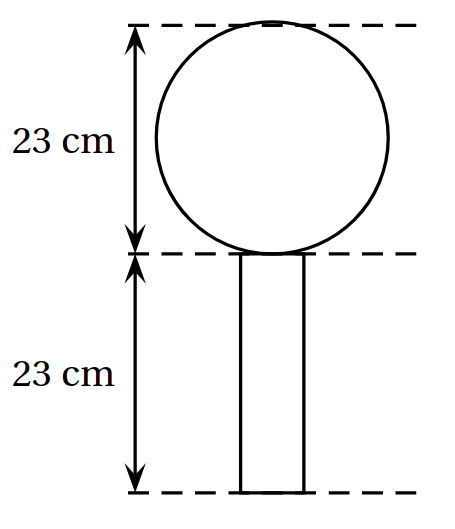
\includegraphics[width=0.8\linewidth]{3x3-volumes-1/sources/globe.png}
  \end{figure}
\end{multicols}

\newpage

\subsubsection*{Exercice 5 - Centrale}

\begin{multicols}{2}
  La centrale géothermique de Rittershoffen (Bas Rhin) a été inaugurée le 7 juin 2016. On y acreusé un puits pour capter de l’eau chaude sous pression, à 2500 m de profondeur, à unetempérature de 170 degrés Celsius. \\
  Ce puits a la forme du tronc de cône représenté ci-contre. \\
  Les proportions ne sont pas respectées.On calcule le volume d’un tronc de cône grâce à la formule suivante : 

  $$ V = \dfrac{1}{3} \times \pi \times h \times (R^2 + R \times r + r^2)$$

  où $h$ désigne la hauteur du tronc de cône, $R$ le rayon de la grande base et $r$ le rayon de la petite base.

  \begin{enumerate}
  \item Vérifier que le volume du puits est environ égal à $225 m^3$
  \item La terre est tassée quand elle est dans le sol. Quand on l’extrait, elle n’est plus tassée et son volume augmente de 30\%. Calculer le volume final de terre à stocker après le forage du puits.
  \end{enumerate}

  \begin{figure}[H]
        \centering
        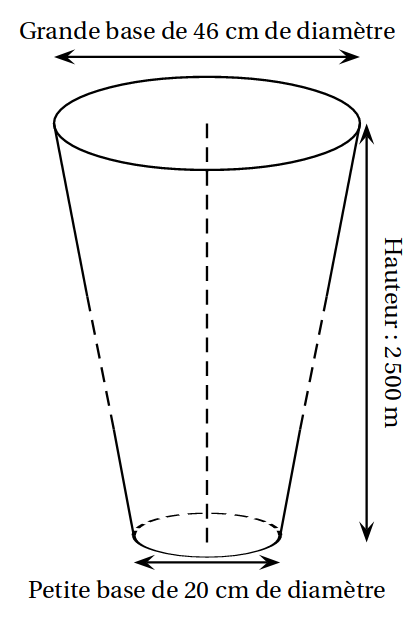
\includegraphics[width=0.8\linewidth]{3x3-volumes-1/sources/boue.png}
  \end{figure}
\end{multicols}


\subsubsection*{Exercice 6 - Yourte}

Samia vit dans un appartement dont la surface au sol est de $35 m^2$. Elle le compare avec une yourte, l’habitat traditionnel mongol

\begin{figure}[H]
      \centering
      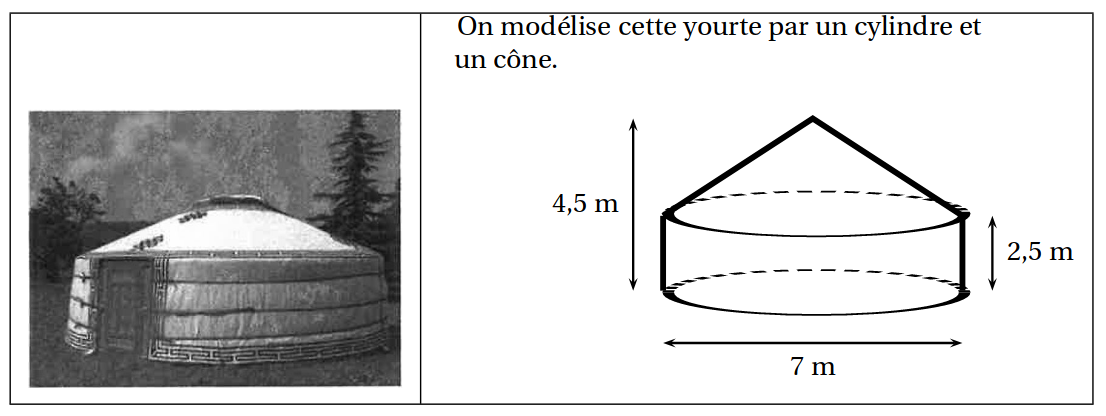
\includegraphics[width=0.8\linewidth]{3x3-volumes-1/sources/yourte.png}
\end{figure}

\begin{enumerate}
\item Montrer que l’appartement de Samia offre une plus petite surface au sol que celle de la yourte.
\item Calculer le volume de la yourte en m3.
\item Sarnia réalise une maquette de cette yourte à l’échelle125.Quelle est la hauteur de la maquette?
\end{enumerate}
  
Rappels : 

\begin{itemize}
  \item Aire du disque = $\pi \times rayon^2$
  \item Volume du cylindre = $\pi \times rayon^2 \times hauteur$
  \item Volume du cône = $\dfrac{1}{3} \times \pi \times rayon^2 \times hauteur$
\end{itemize}

\newpage

\subsubsection*{Exercice 7 - Solides}

Voici les dimensions de quatre solides :

\begin{itemize}
\item Une pyramide de 6 cm de hauteur dont la base est un rectangle de 6 cm de longueur et de 3 cm de largeur.
\item Un cylindre de 2 cm de rayon et de 3 cm de hauteur.
\item Un cône de 3 cm de rayon et de 3 cm de hauteur.
\item Une boule de 2 cm de rayon.
\end{itemize}

\begin{enumerate}
\item Représenter approximativement les trois premiers solides avec leur taille réelle. Placer les dimensions données sur les représentations.
\item Classer ces quatre solides dans l’ordre croissantde leur volume.\\
\end{enumerate}

Rappels : 

\begin{itemize}
  \item $\dfrac{4}{3} \times \pi  \times rayon^3$
  \item $\pi  \times rayon^2  \times hauteur $
  \item $\dfrac{1}{3} \times \pi \times rayon^2 \times hauteur$
  \item $\dfrac{1}{3} \times \text{aire de la base} \times hauteur$
\end{itemize}

\subsubsection*{Exercice 8 - Sauce}

\begin{multicols}{2}

  Dans le village de Jean, une brocante est organisée chaque année lors du premier week-end de juillet. Jean s’est engagé à s’occuper du stand de vente de frites. Pour cela, il fabrique des cônes en papier qui les vendre. \\
  Dans le fond de chaque cône, Jean versera de la sauce : soit de la mayonnaise, soit de la sauce tomate. 
  Il décide de fabriquer 400 cônes en papier et il doit estimer le nombre de bouteilles de mayonnaise et de sauce tomate à acheter pour ne pas en manquer. \\

  Les acheteurs : 80 \% des acheteurs prennent de la sauce tomate et tous les autres prennent de la mayonnaise. Les sauces:La bouteille de mayonnaise est assimilée à un cylindre de révolution dont le diamètre de base est 5 cm et la hauteur est 15 cm. La bouteille de sauce tomate a une capacité de 500 mL.

  \begin{enumerate}
  \item Montrer que le volume de sauce pour un cône de frites est d’environ 11,78 cm3
  \item Déterminer le nombre de bouteilles de chaque sauce que Jean devra acheter. \\
    \textit{Laisser toute trace de recherche, même si elle n’est pas aboutie.} \\
  \end{enumerate}

  Voici les informations dont Jean dispose pour faire ses calculs :

  \begin{figure}[H]
        \centering
        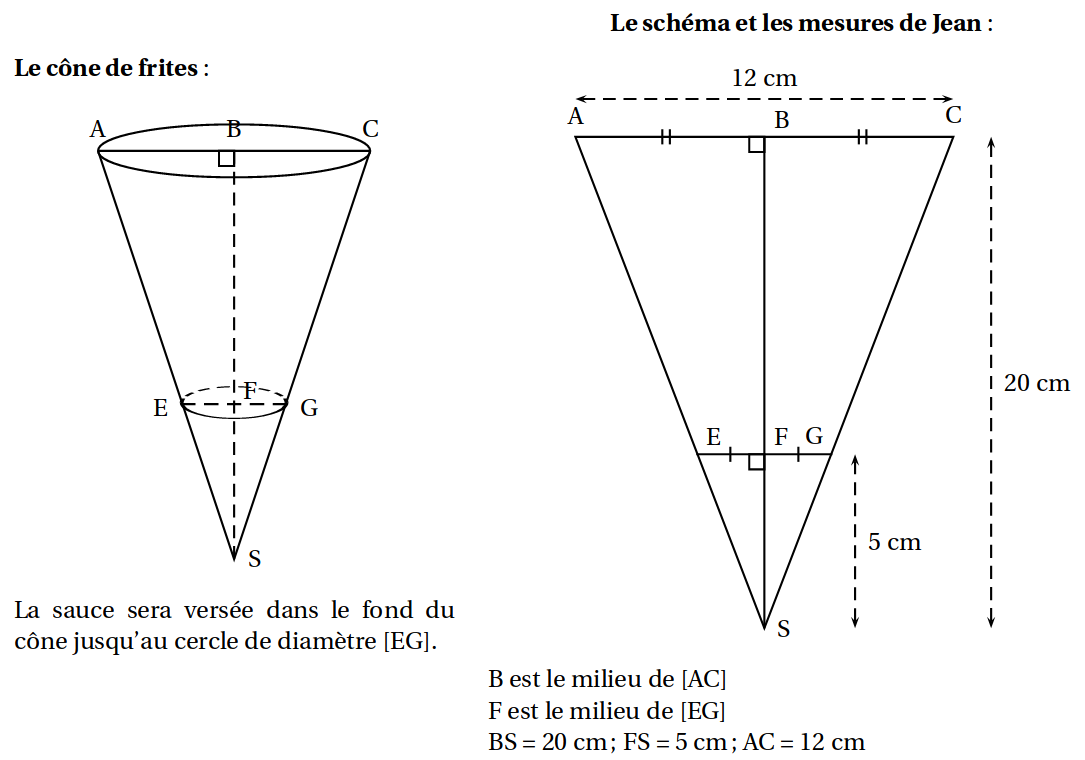
\includegraphics[width=\linewidth]{3x3-volumes-1/sources/sauce.png}
  \end{figure}
  Rappels : 

  \begin{itemize}
  \item Volume d’un cône : $\dfrac{1}{3} \times \pi \times rayon^2 \times hauteur$
  \item Volume d’un cylindre : $\pi \times rayon^2 \times hauteur$
  \item $1000 cm^3 = 1 Litre$
  \end{itemize}

\end{multicols}

\newpage

\subsubsection*{Exercice 9 - Escalier}

\begin{multicols}{2}

  Afin de faciliter l'accès à sa piscine, Monsieur Joseph décide de construire un escalier constitué de deux prismes superposés dont les bases sont des triangles rectangles.

  \begin{enumerate}
  \item Démontrer que le volume de l'escalier est égal à $1,26208 m^3$.
  \item Sachant que l'escalier est un ouvrage en béton courant, déterminer le nombre de sacs de ciment de 35 kg nécessaires à la réalisation de l'escalier.
  \item Déterminer la quantité d'eau nécessaire à cet ouvrage.
  \end{enumerate}

  \begin{figure}[H]
        \centering
        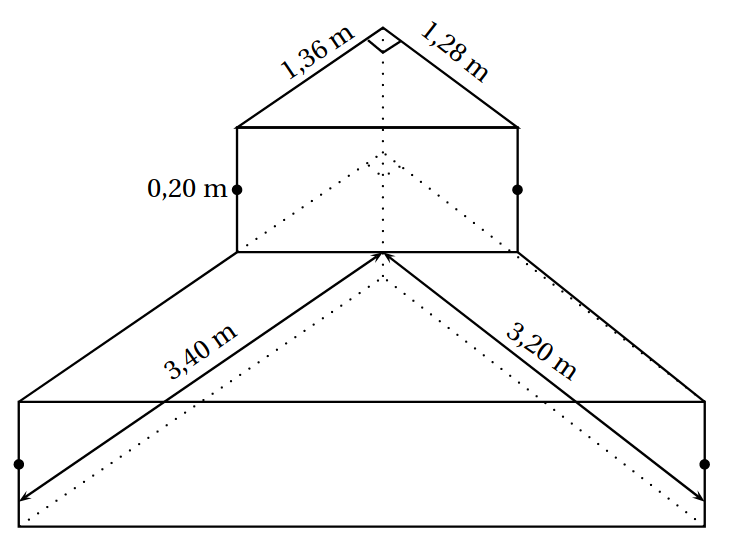
\includegraphics[width=\linewidth]{3x3-volumes-1/sources/escalier.png}
  \end{figure}


\end{multicols}

\textbf{Information 1 :} Volume du prisme = aire de la base $\times$ hauteur ;\quad  1~L = 1~dm$^3$

\textbf{Information 2 :} Voici la reproduction d'une étiquette figurant au dos d'un sac de ciment
de 35~kg.

\begin{center}
  \begin{tabular}{|c|c|c|c|c|}  \hline
    Dosage pour 1 sac de 35 kg	&Volume de béton obtenu	&Sable (seaux)	&Gravillons (seaux)	&Eau\\ \hline
    Mortier courant 			&105 L					&10				&					&16 L\\ \hline
    Ouvrages en béton courant	&100 L					&5				&8 					&17 L\\ \hline
    Montage de murs 			&120 L 					&12				&					&18~L\\ \hline
  \end{tabular}
\end{center}
\textit{Dosages donnés à titre indicatif et pouvant varier suivant les matériaux régionaux et le taux d'hygrométrie des granulats}

\subsubsection*{Exercice 10 - Piscine}

Une famille désire acheter, pour les enfants, une piscine cylindrique hors sol équipée d’une pompe électrique. Elle compte l’utiliser cet été du mois de juin au mois de septembre inclus. Elle dispose d’un budget de 200\euro. \\
À l’aide des documents suivants, dire si le budget de cette famille est suffisant pour l’achat de cettepiscine et les frais de fonctionnement. \\
\textit{Laisser toute trace de recherche, même si elle n’est pas aboutie.}
z
\begin{figure}[H]
      \centering
      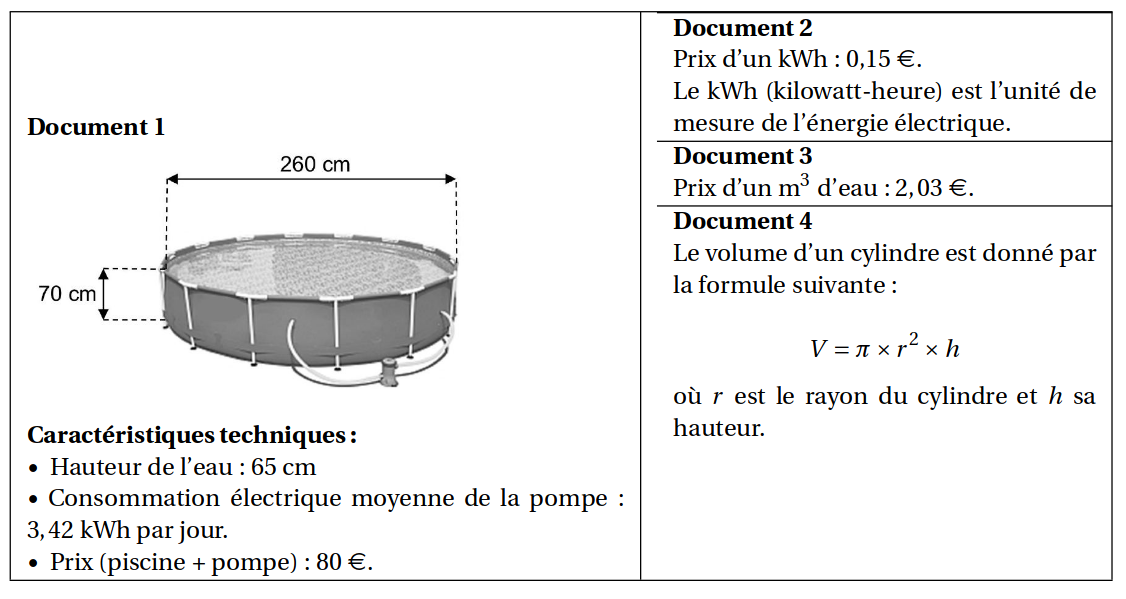
\includegraphics[width=0.8\linewidth]{3x3-volumes-1/sources/piscine.png}
\end{figure}

\end{document}
